\documentclass[12pt]{article}
\usepackage[paper=letterpaper,margin=2cm]{geometry}
\usepackage{amsmath}
\usepackage{amssymb}
\usepackage{amsfonts}
\usepackage{newtxtext, newtxmath}
\usepackage{enumitem}
\usepackage{titling}
\usepackage{multirow}
\usepackage{textcomp}
\usepackage{graphicx}
\usepackage{tikz}
\usepackage{listings}
\usepackage{xcolor}
\graphicspath{ {./images/} }

\definecolor{codegreen}{rgb}{0,0.6,0}
\definecolor{codegray}{rgb}{0.5,0.5,0.5}
\definecolor{codepurple}{rgb}{0.58,0,0.82}
\definecolor{backcolour}{rgb}{0.95,0.95,0.92}

\lstdefinestyle{mystyle}{
    backgroundcolor=\color{backcolour},   
    commentstyle=\color{codegreen},
    keywordstyle=\color{magenta},
    numberstyle=\tiny\color{codegray},
    stringstyle=\color{codepurple},
    basicstyle=\ttfamily\footnotesize,
    breakatwhitespace=false,         
    breaklines=true,                 
    captionpos=b,                    
    keepspaces=true,                 
    numbers=left,                    
    numbersep=5pt,                  
    showspaces=false,                
    showstringspaces=false,
    showtabs=false,                  
    tabsize=2
}

\lstset{style=mystyle}

\newdimen\nodeDist
\nodeDist=35mm
\usetikzlibrary{positioning}
\usepackage[colorlinks=true]{hyperref}

\setlength{\droptitle}{-6em}

\title{\large{Aprendizagem 2022}\vskip 0.2cm Homework II -- Group 58}
\date{}
\begin{document}
\maketitle
\center\large{\vskip -2.5cm\textbf{Part I}: Pen and paper}
\begin{enumerate}[leftmargin=\labelsep]


\item \leavevmode\vadjust{\vspace{-\baselineskip}}
\begin{center}
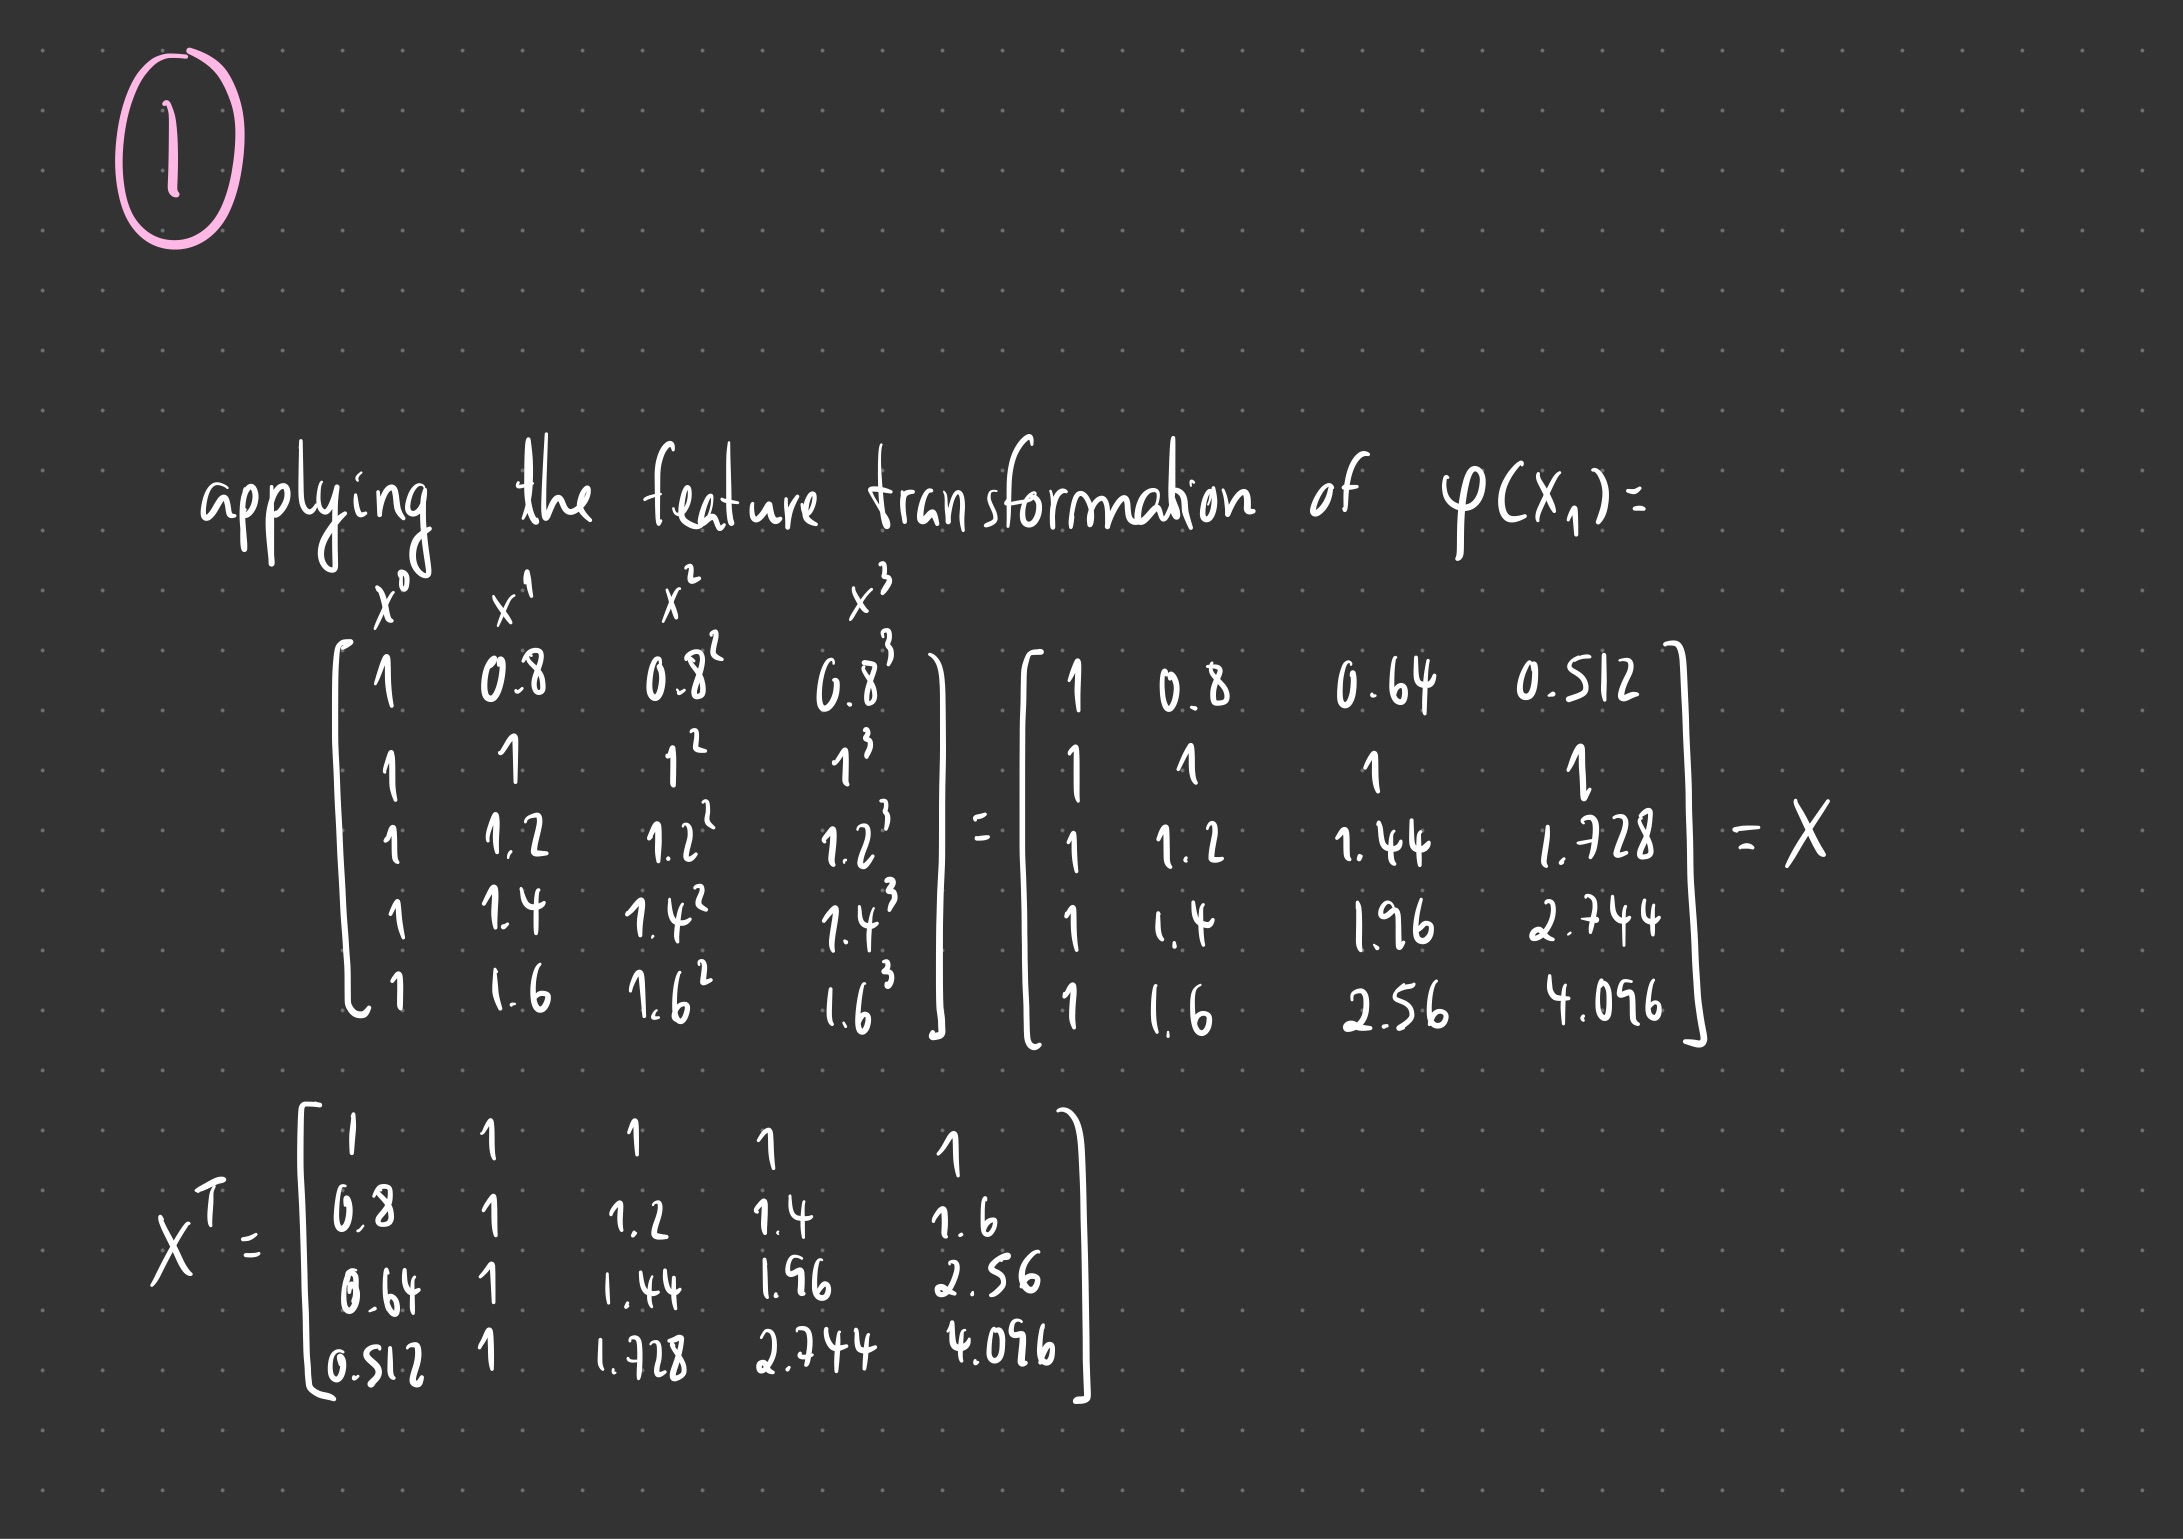
\includegraphics[scale=0.2]{images/Project-31.jpg}
\newline
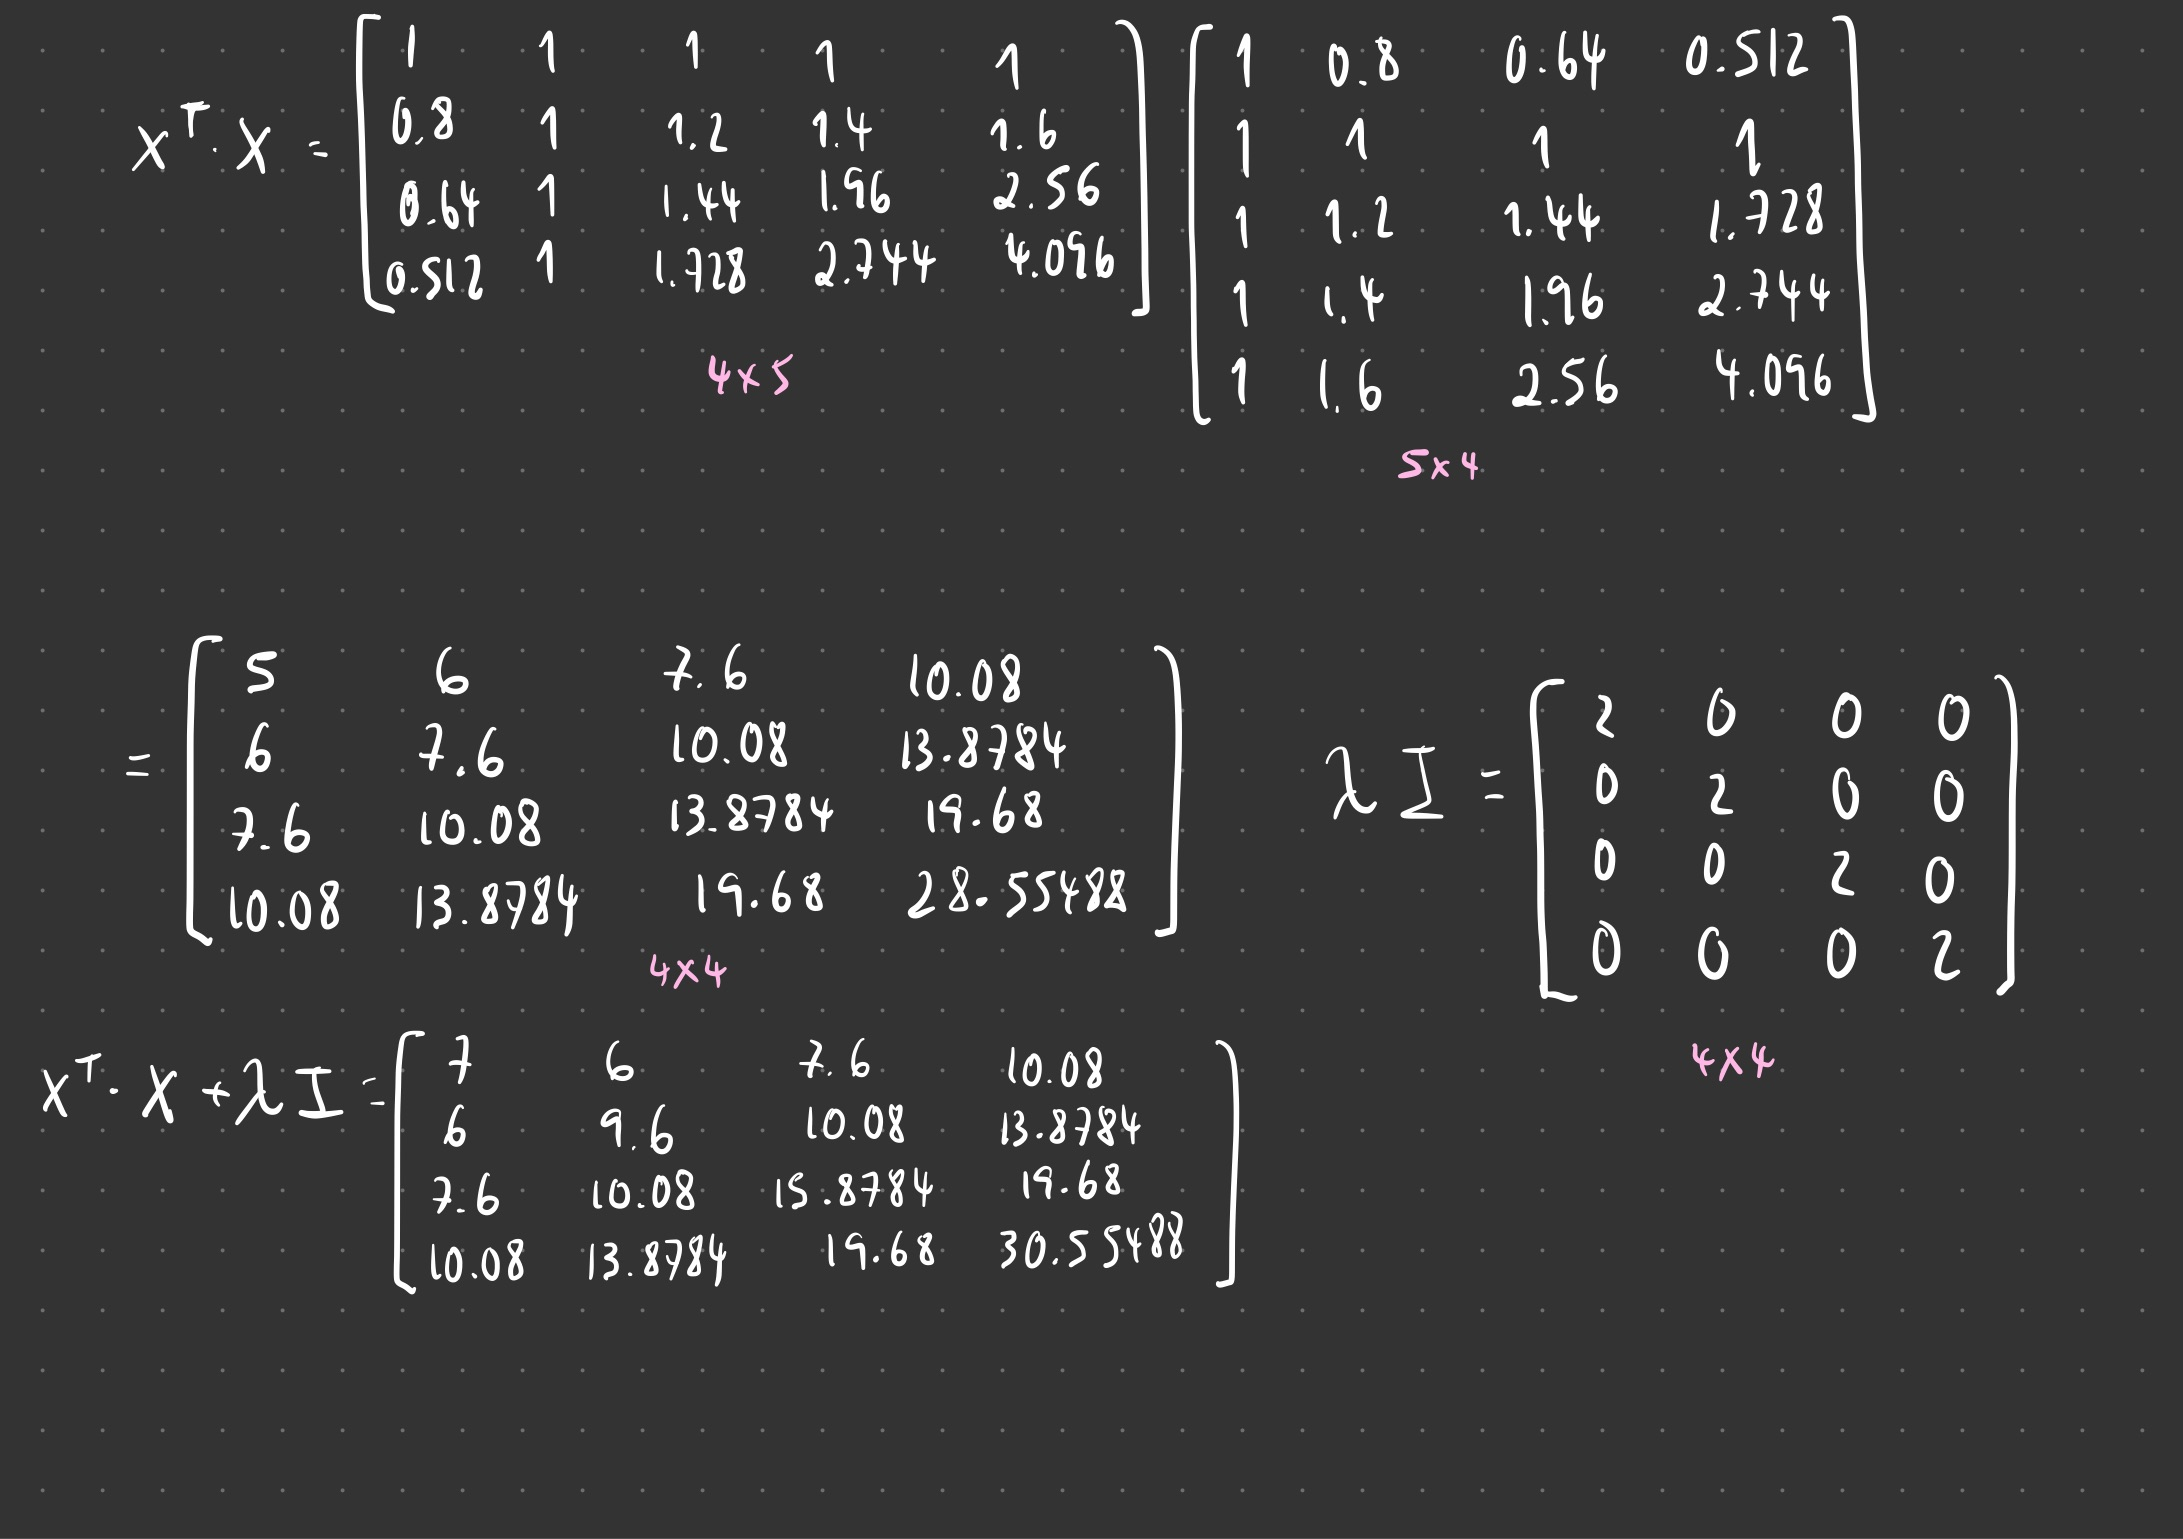
\includegraphics[scale=0.2]{images/Project-32.jpg}
\newline
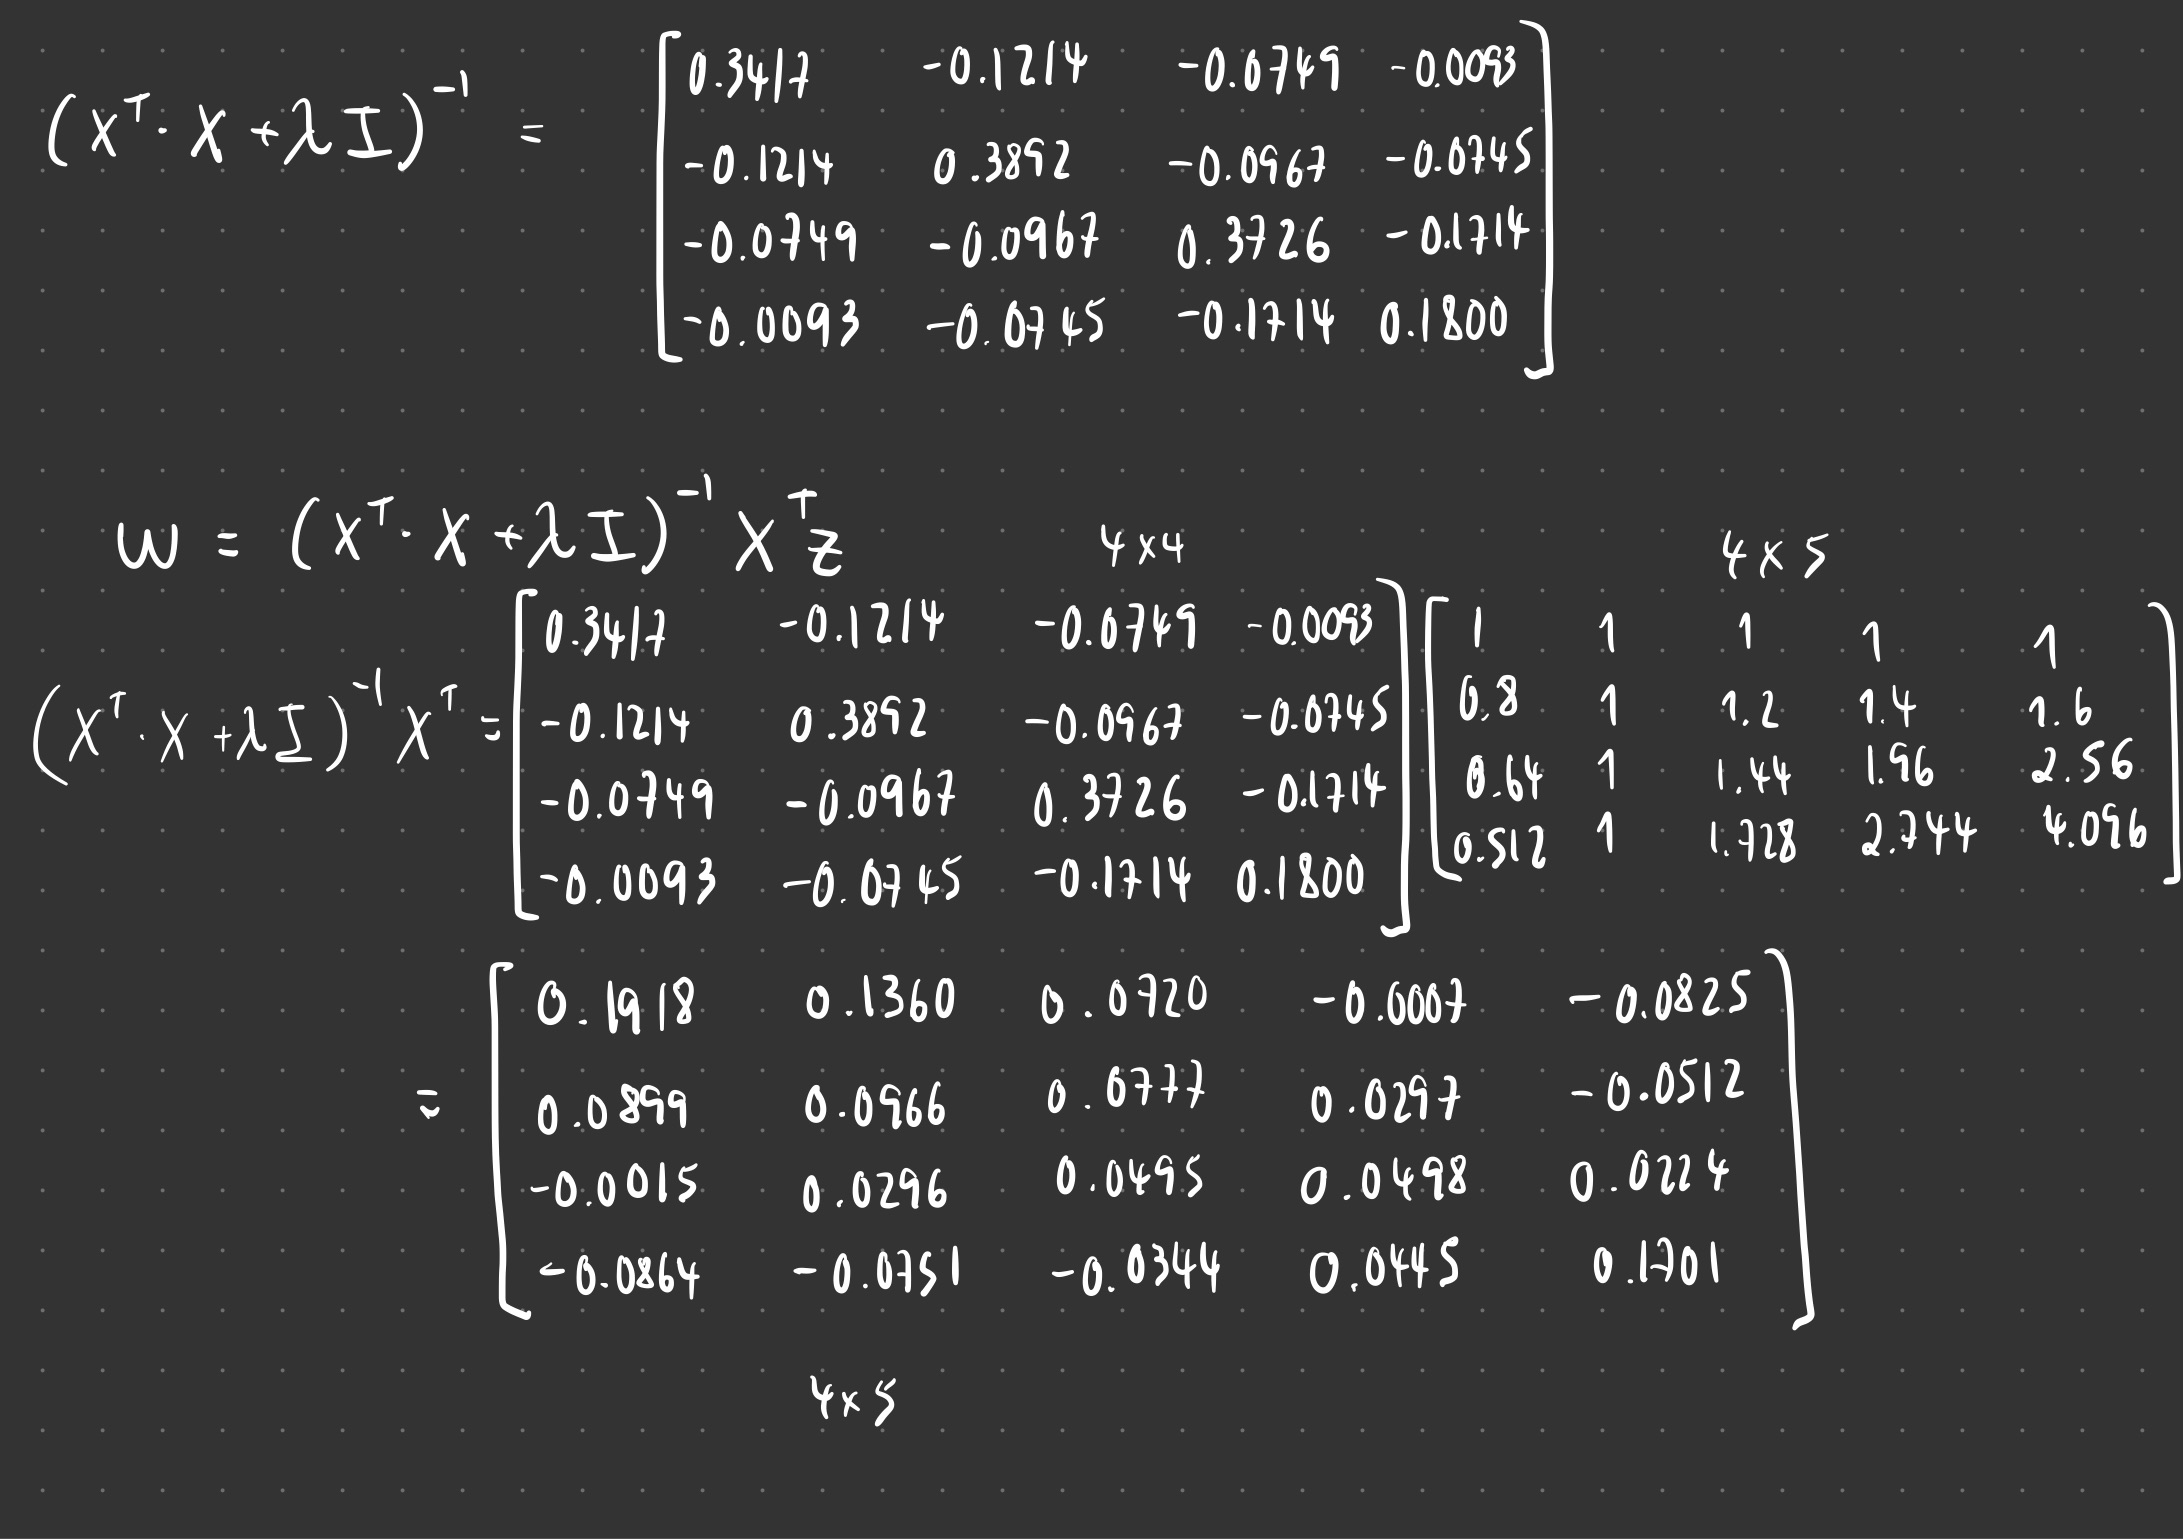
\includegraphics[scale=0.2]{images/Project-33.jpg}
\newline
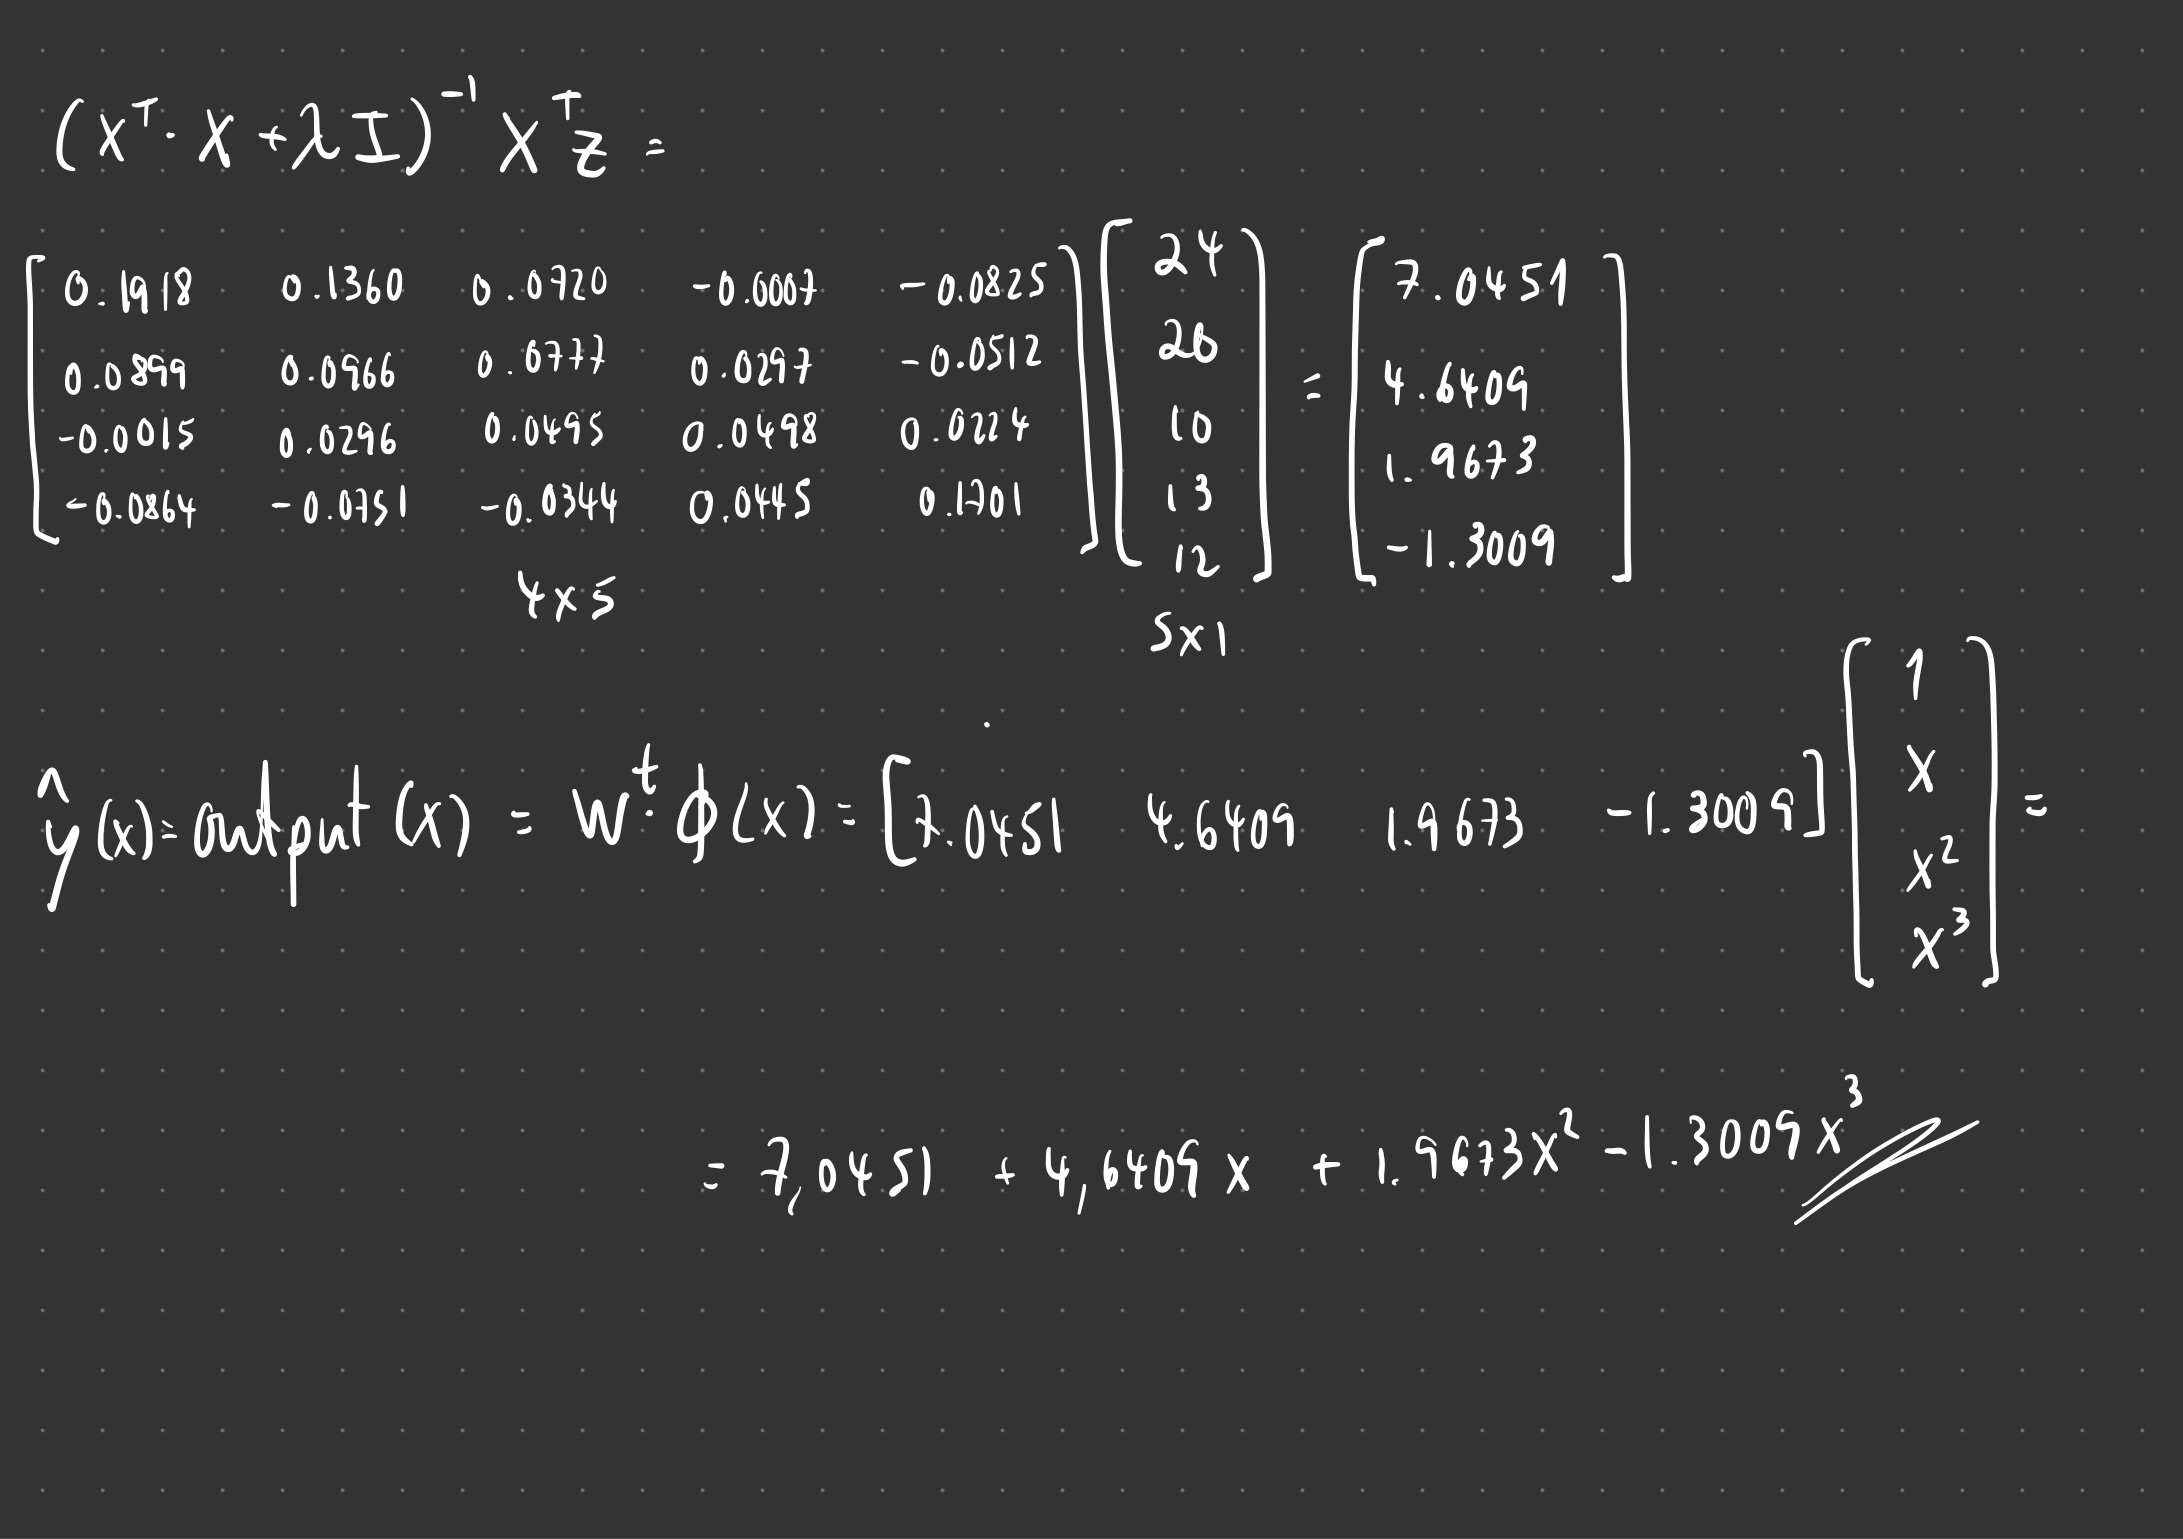
\includegraphics[scale=0.2]{images/Project-34.jpg}
\newline
\end{center}
\newpage

\item \leavevmode\vadjust{\vspace{-\baselineskip}}
\begin{center}
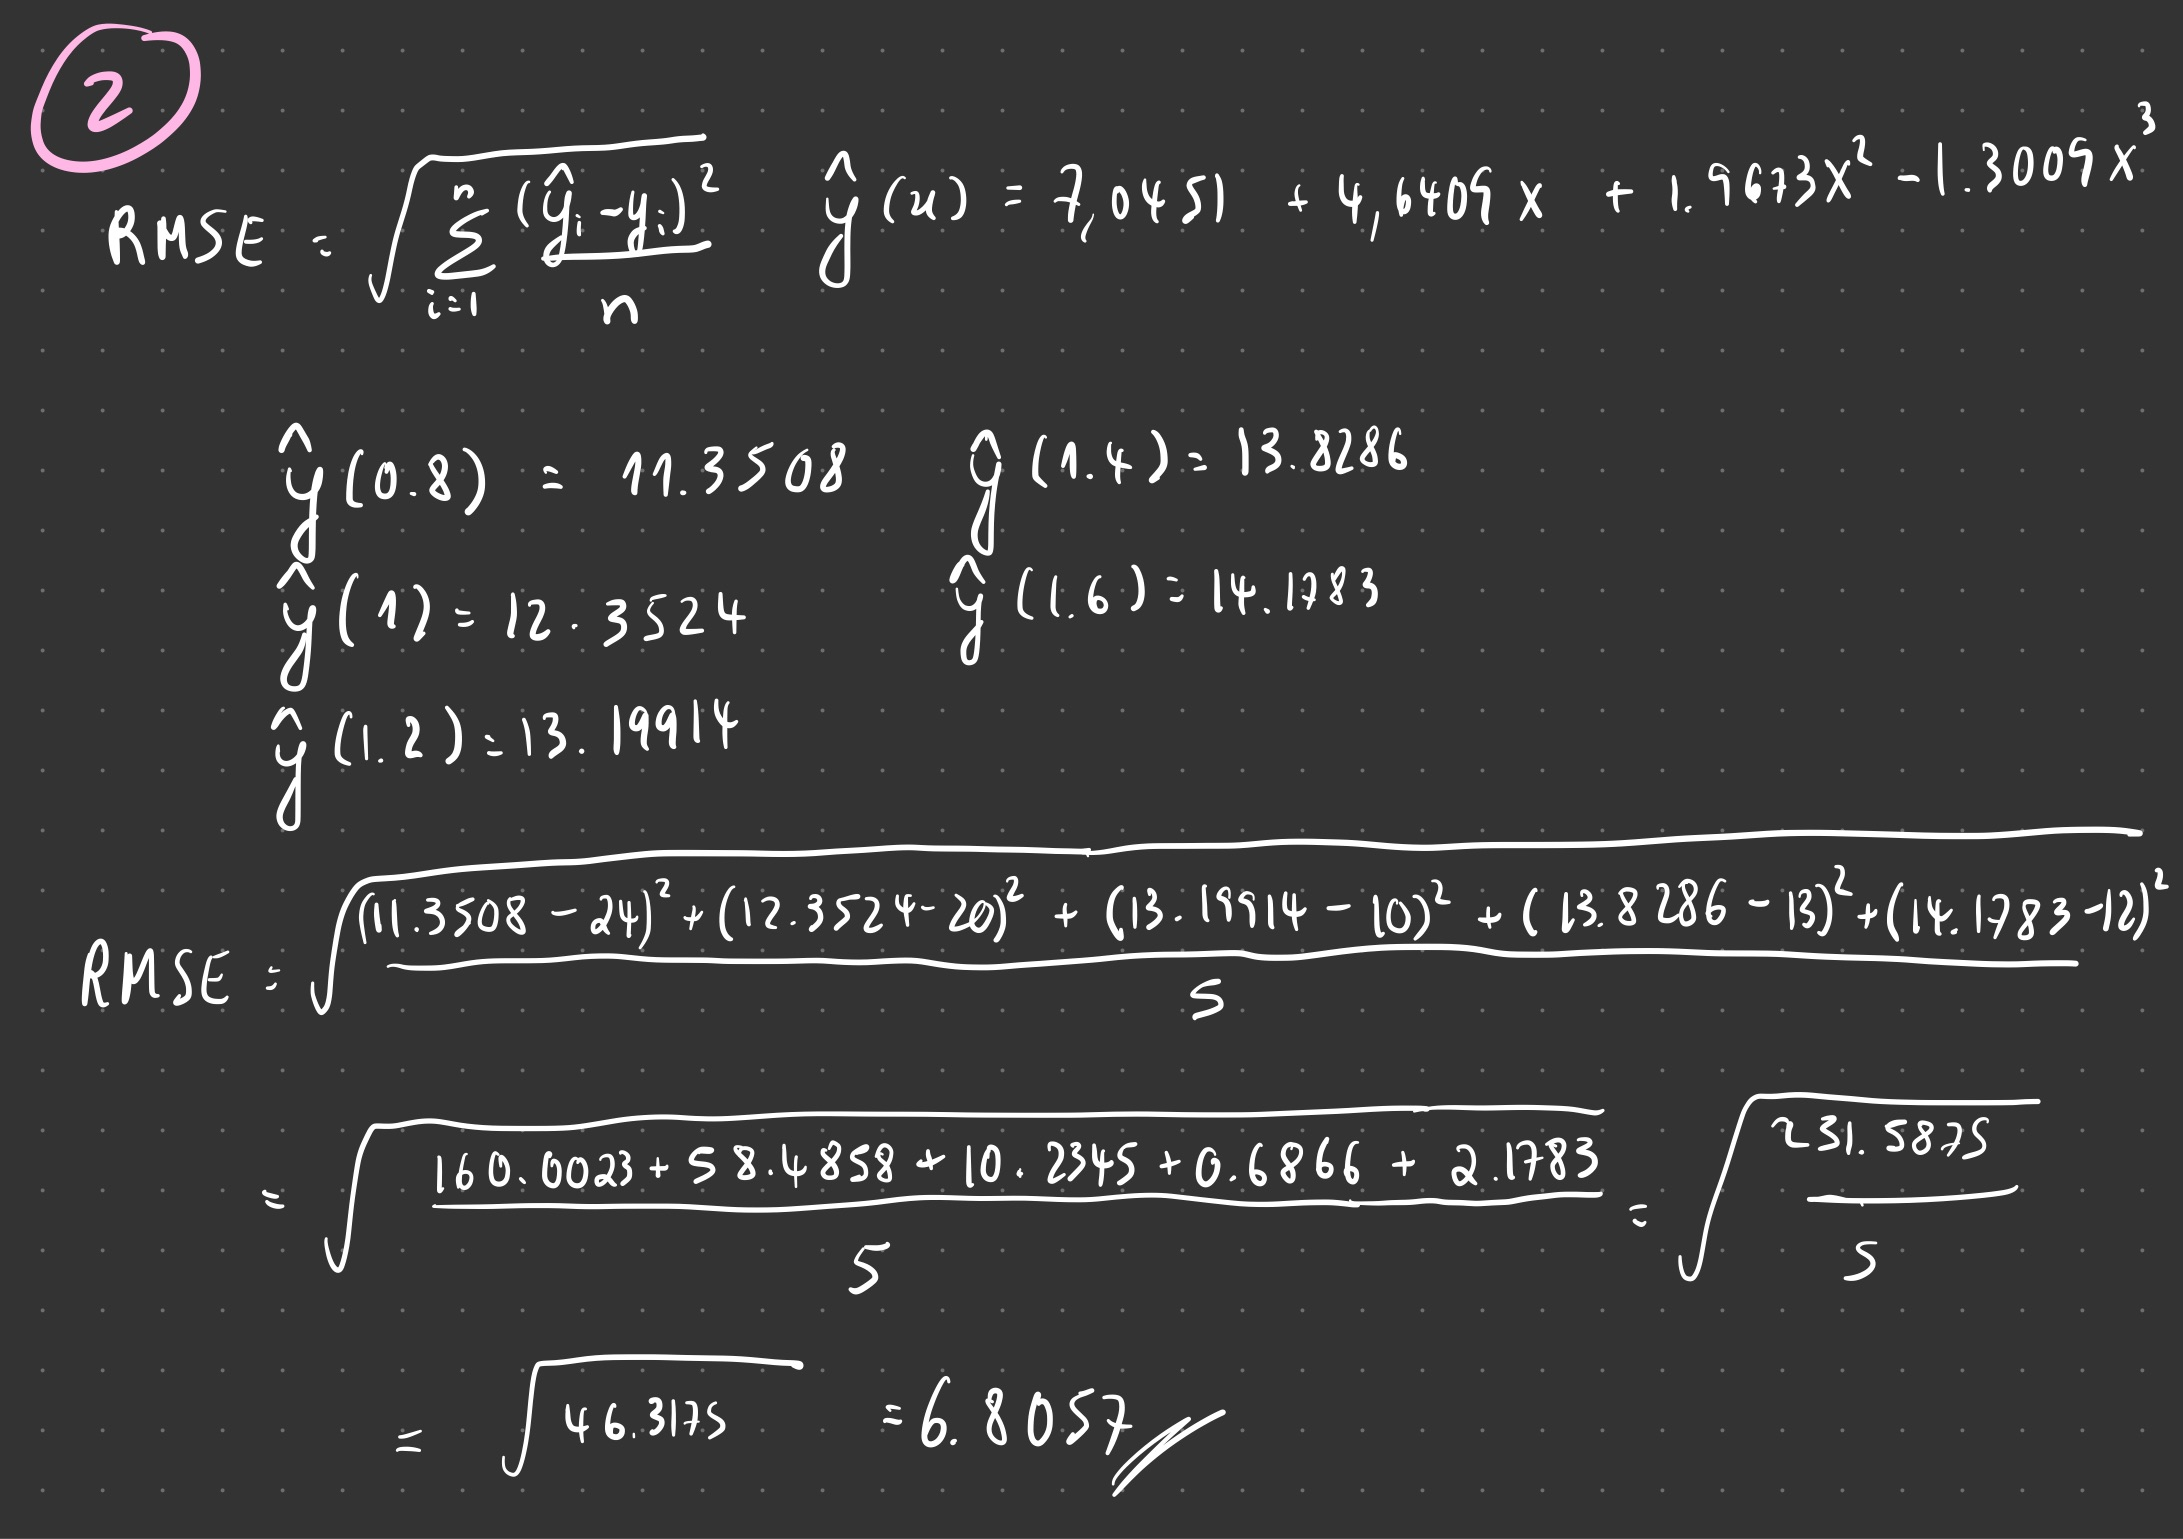
\includegraphics[scale=0.2]{images/Project-35.jpg}
\newline
\end{center}
\newpage
\item \leavevmode\vadjust{\vspace{-\baselineskip}}
\begin{center}
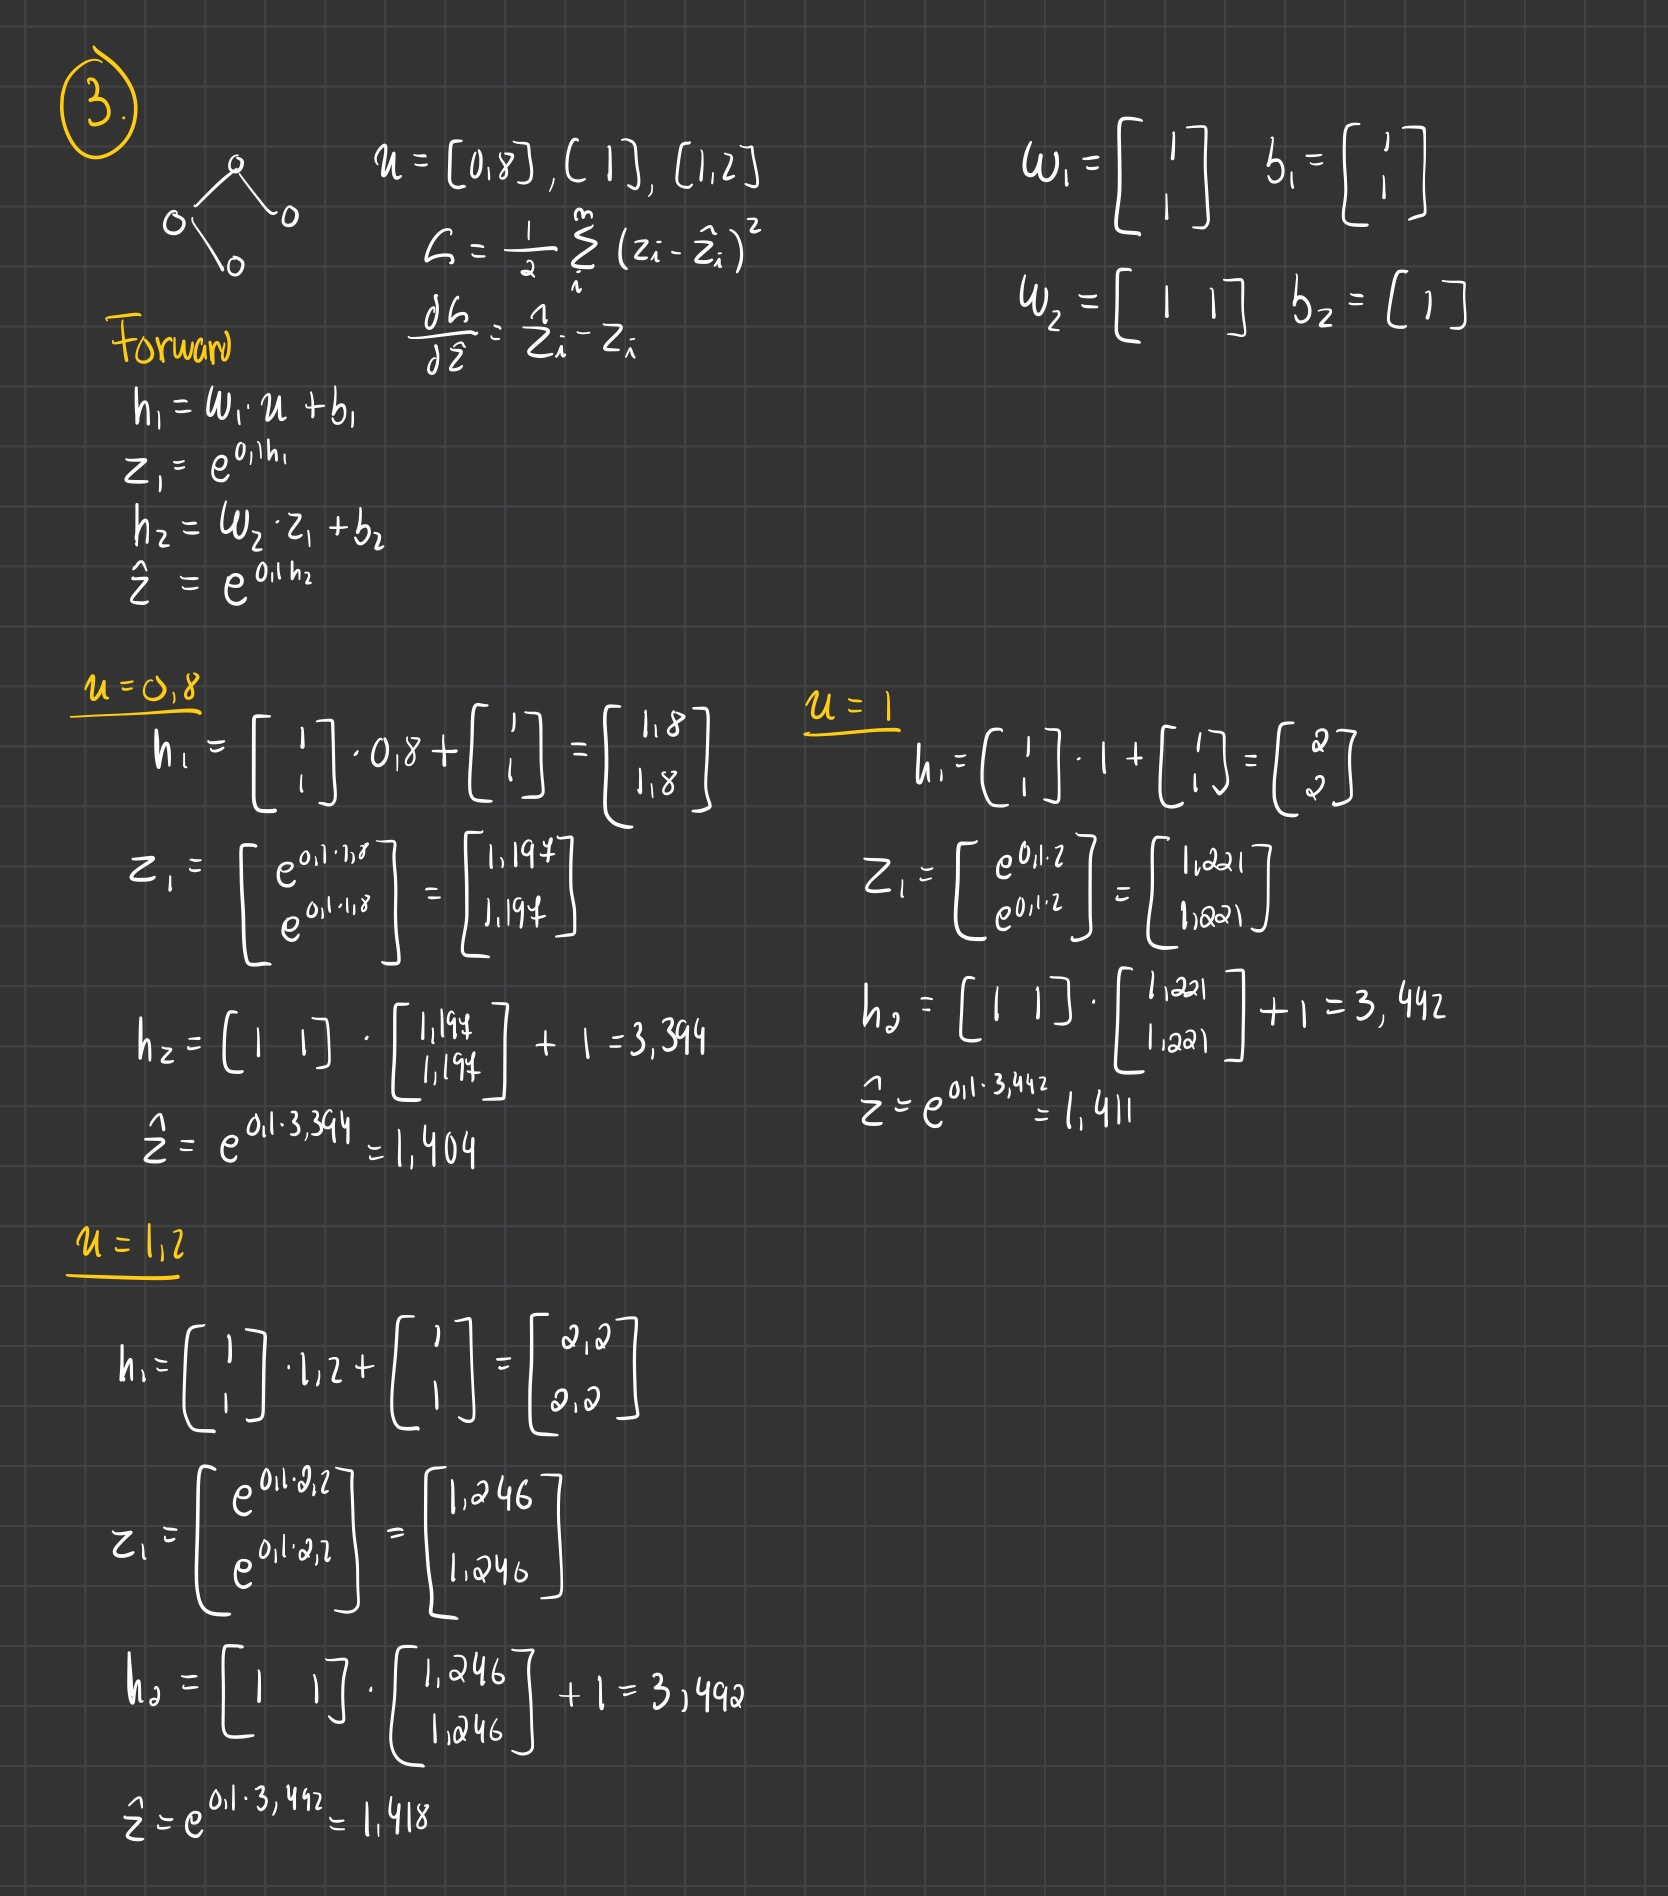
\includegraphics[scale=0.3]{images/hw3-1.jpg}
\newline
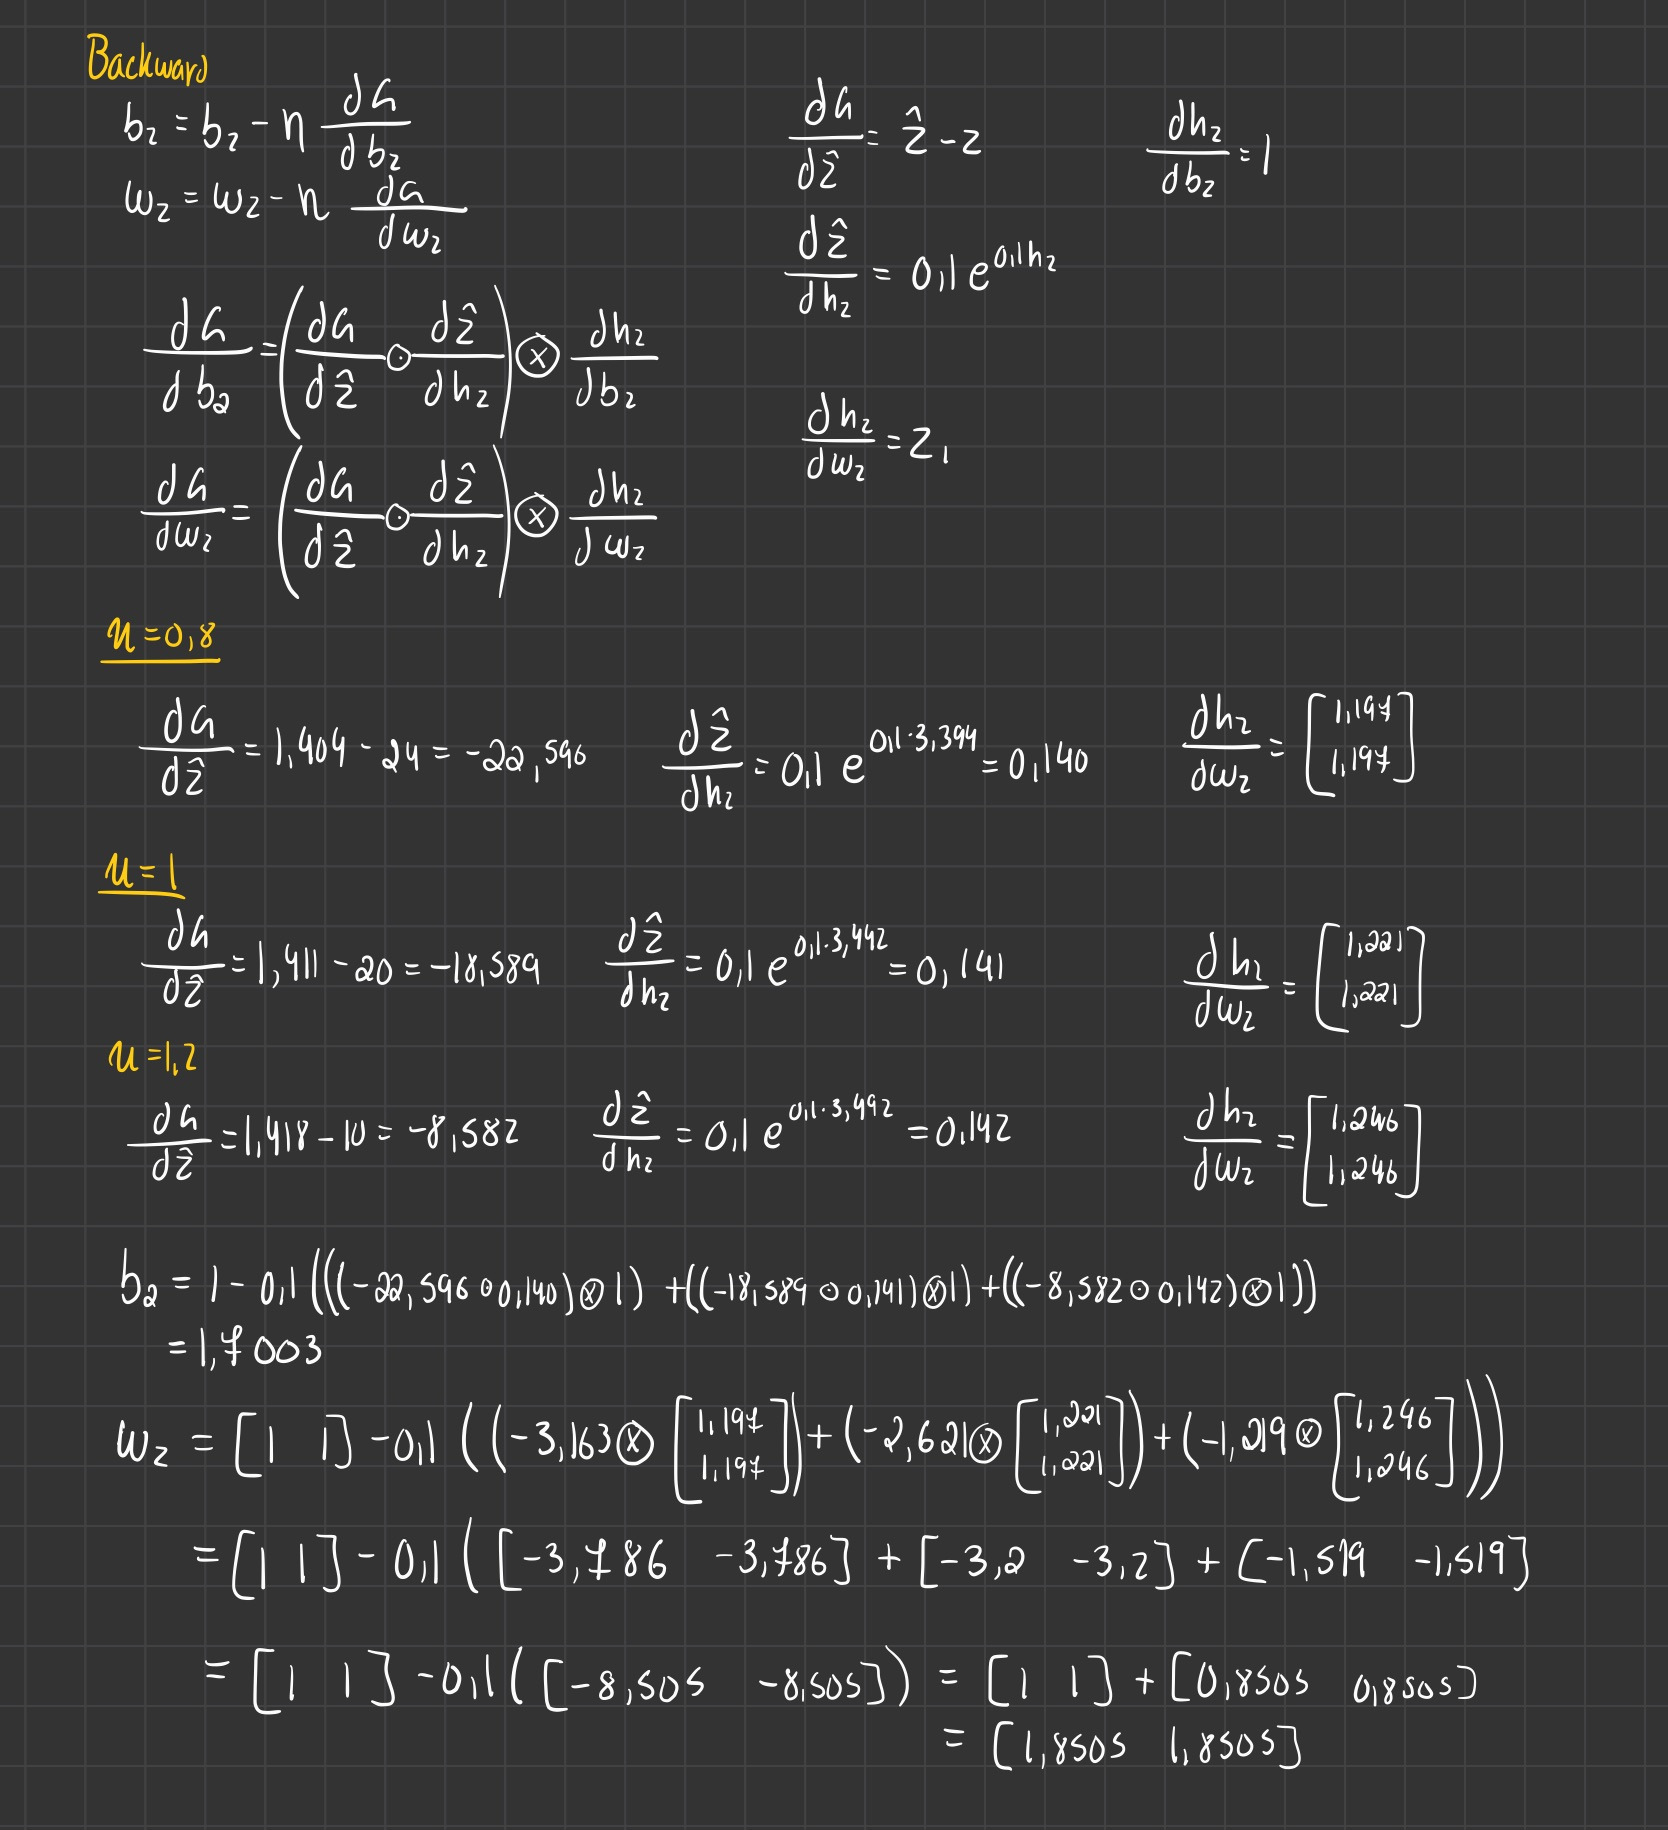
\includegraphics[scale=0.3]{images/hw3-2.jpg}
\newline
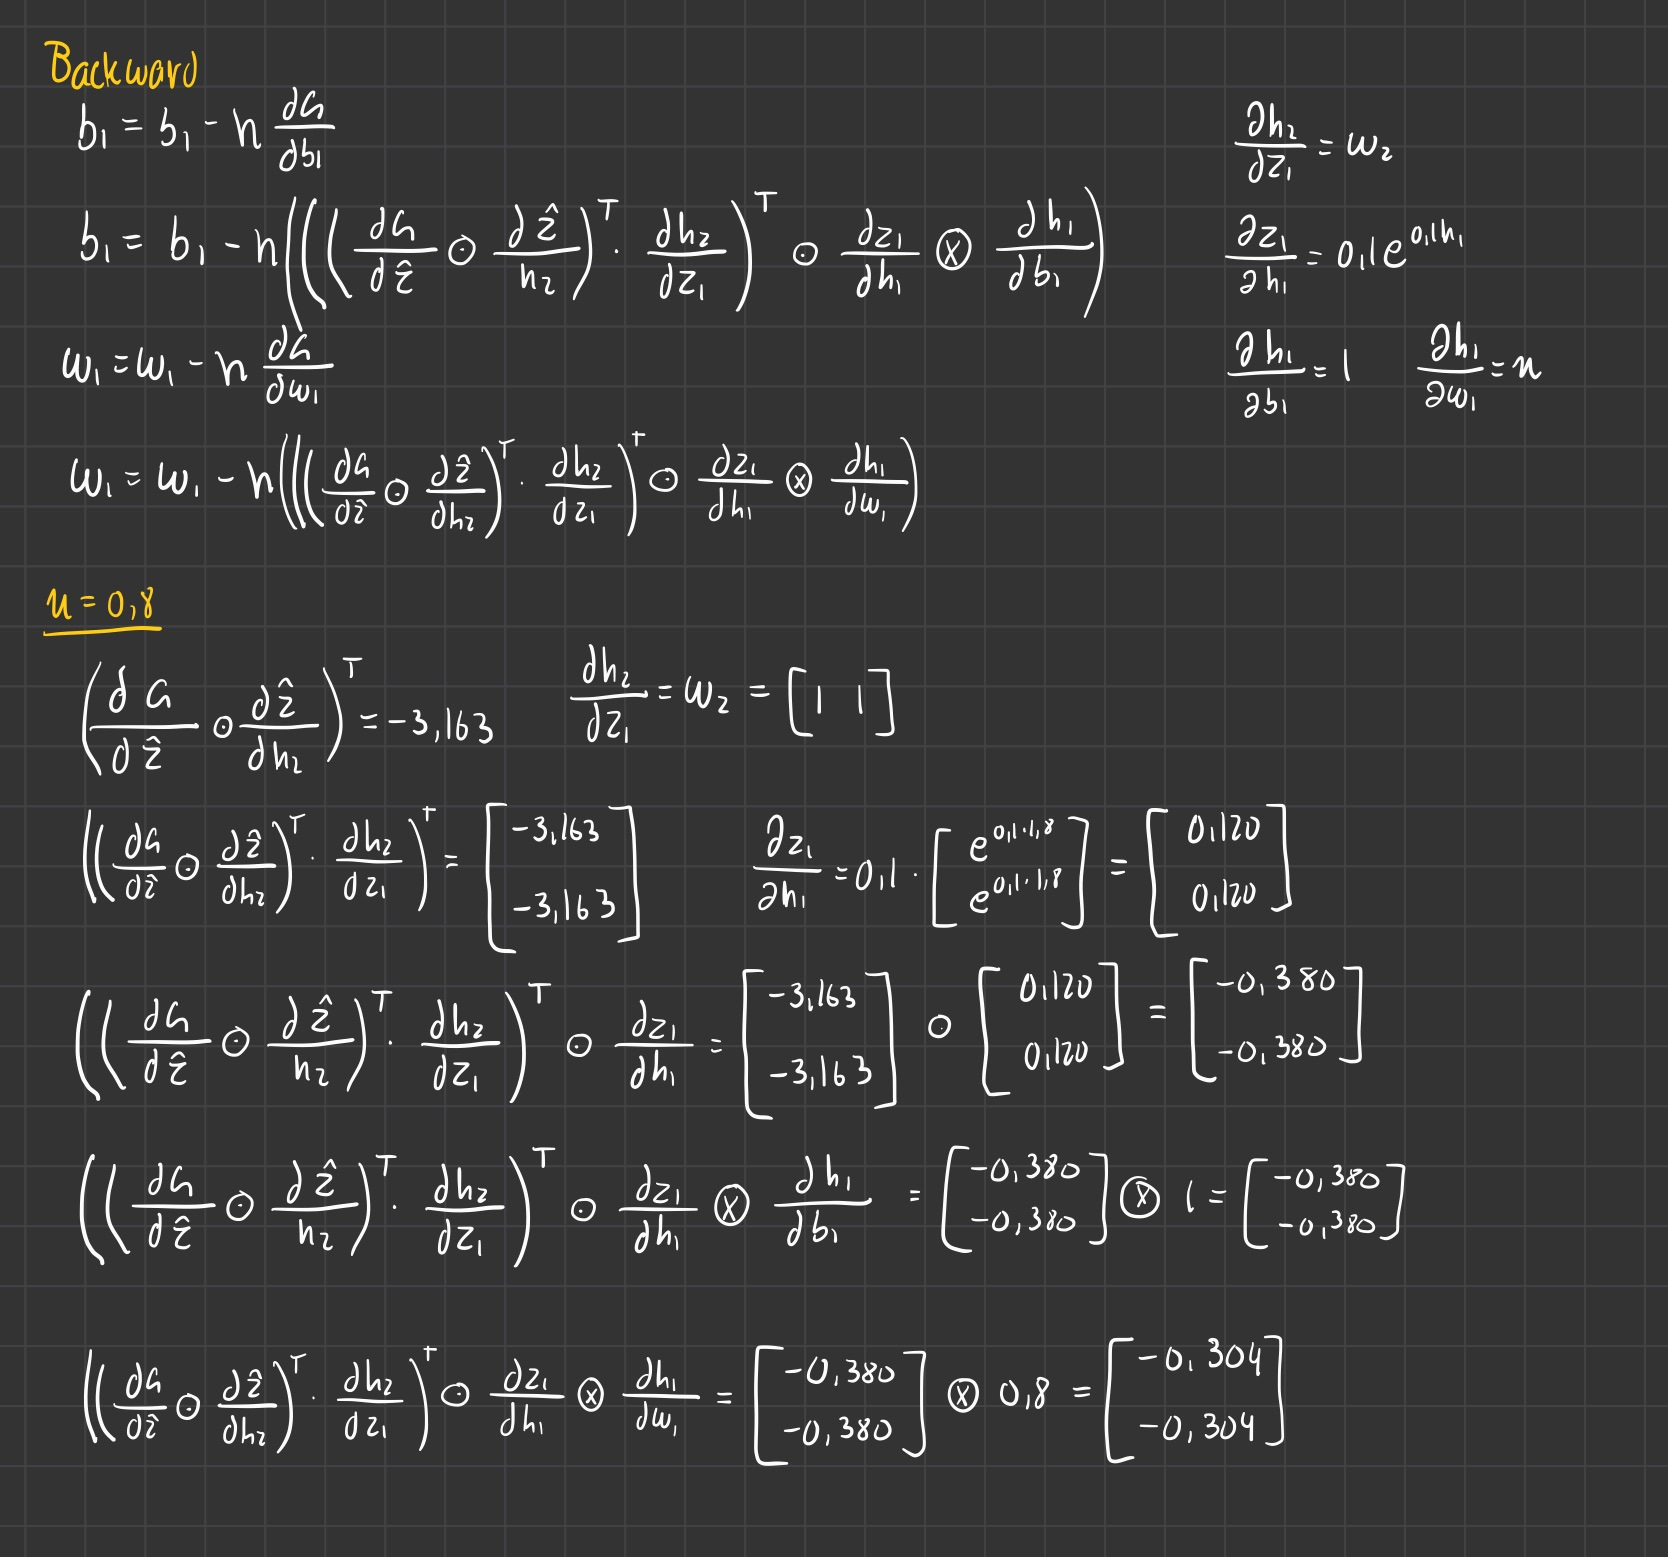
\includegraphics[scale=0.3]{images/hw3-3.jpg}
\newline
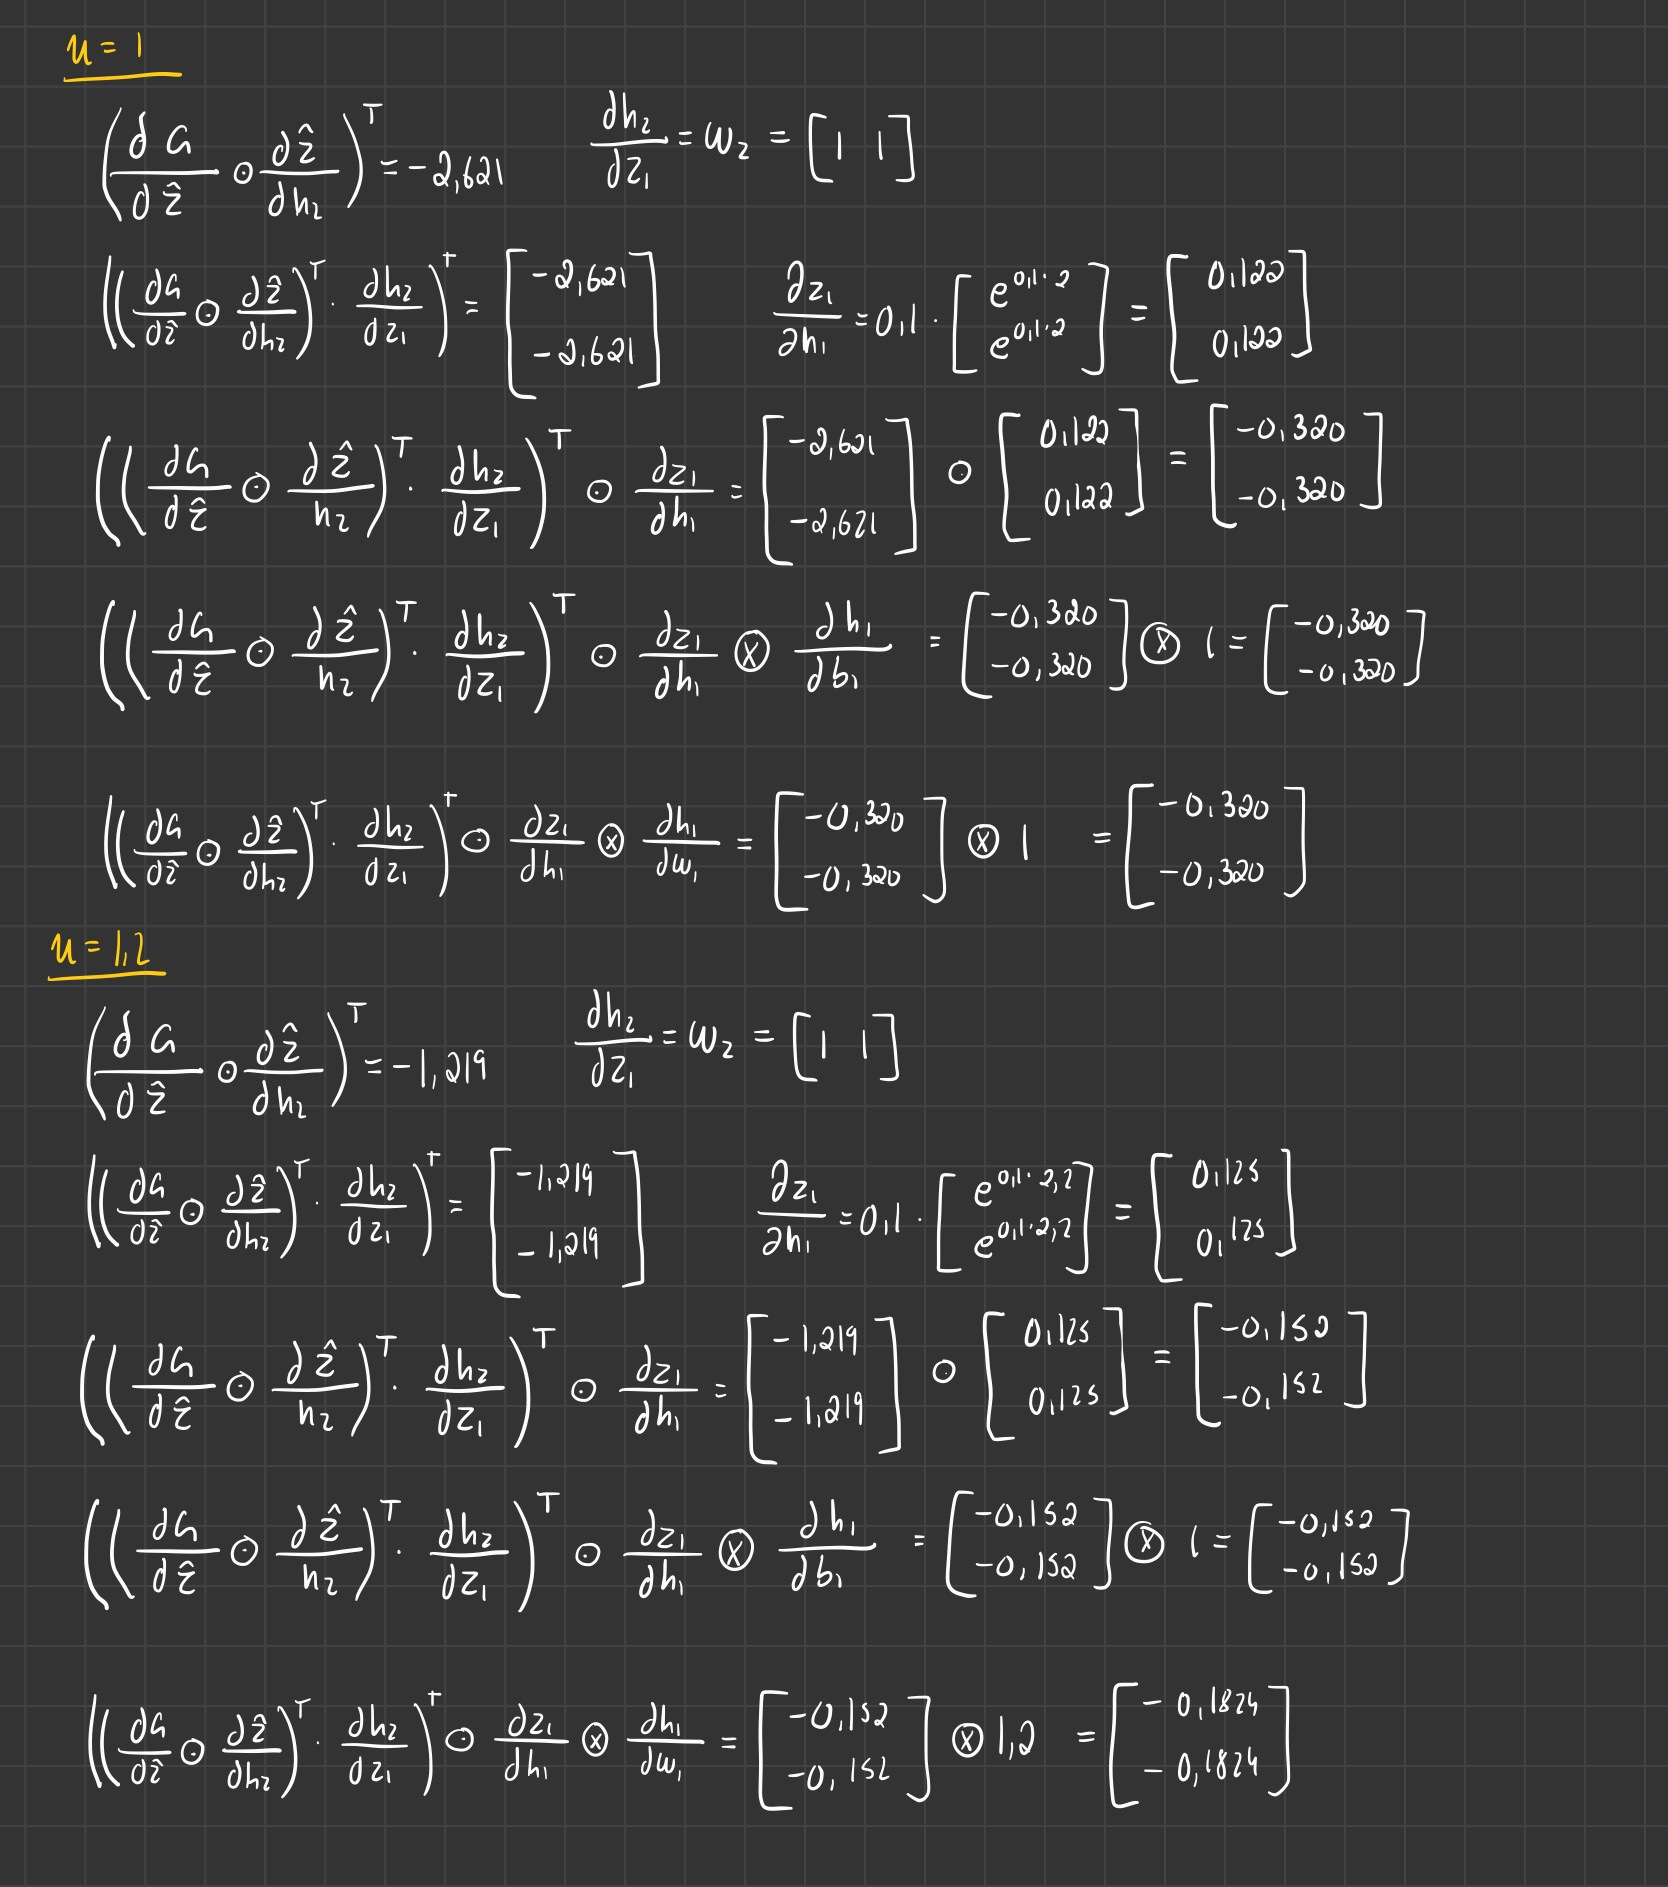
\includegraphics[scale=0.3]{images/hw3-4.jpg}
\newline
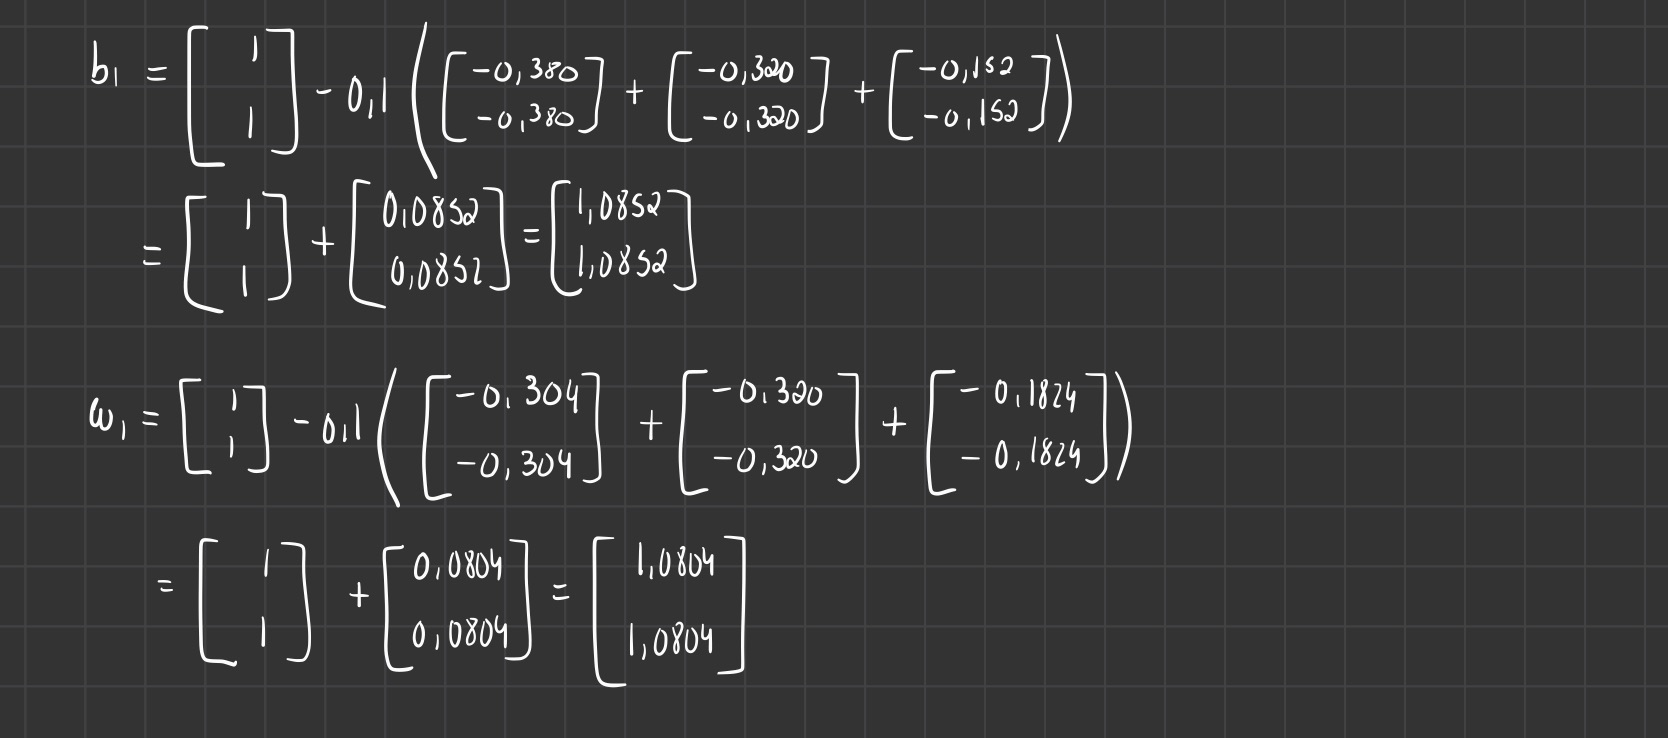
\includegraphics[scale=0.3]{images/hw3-5.jpg}
\newline
\end{center}
\end{enumerate}
\newpage
\center\large{\textbf{Part II}: Programming}

\begin{enumerate}[leftmargin=\labelsep,resume]
\item
$Ridge$ \ MAE: 0.162829976437694 \\
$MLP_1$ \ MAE: 0.0680414073796843 \\
$MLP_2$ \ MAE: 0.0978071820387748

\item 
\leavevmode\vadjust{\vspace{-\baselineskip}}
\begin{center}
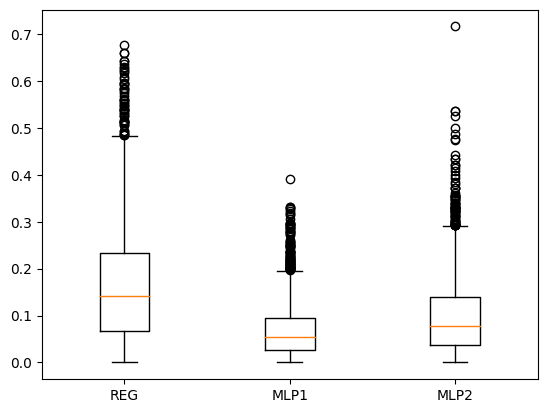
\includegraphics[]{images/boxplot.png}
\newline
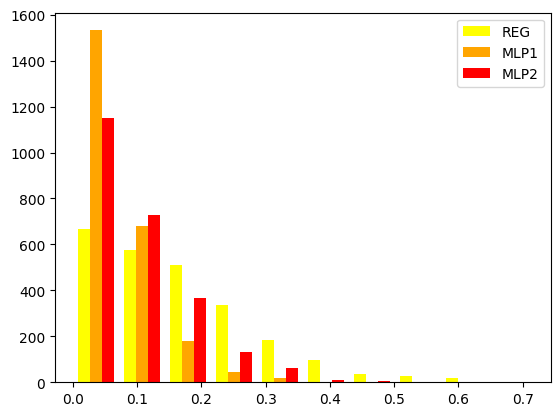
\includegraphics[scale = 0.97]{images/histogram.png}
\end{center}

\item
$MLP_1$ number of iterations: 452 \\
$MLP_2$ number of iterations: 77

\item
We can observe that the Mean Absolute Error of $MLP_1$ is lower thsn the MSE of $MLP_2$ and the number of iterations of $MLP1$ is significantly higher (about 6 times) than those of $MLP_2$. \\
In $MLP_1$, early stopping was considered, which means the training is stopped if the MSE on the validation set becomes bigger, even if the MSE on the training set goes down. In $MPL_1$, the MSE on the validation set (10\% of training data) of our problem only starts growing after 452 iterations, way after the condition to stop when $early\textunderscore stopping = false$ (which is when the loss or score is not improving for $n\textunderscore iter\textunderscore no\textunderscore change$ consecutive iterations) is met.

\end{enumerate}
\newpage
\center\large{\textbf{Appendix}\vskip 0.3cm}

\begin{lstlisting}[language=Python]
import pandas as pd
import numpy as np
import matplotlib.pyplot as plt
from scipy.io.arff import loadarff
from sklearn.linear_model import Ridge
from sklearn.model_selection import train_test_split
from sklearn.metrics import mean_absolute_error
from sklearn.neural_network import MLPRegressor

data = loadarff('kin8nm.arff')
df = pd.DataFrame(data[0])
X = df.drop('y', axis=1)
y = df['y']

X_train, X_test, y_train, y_test = train_test_split(X, y, train_size = 0.7, random_state = 0)

reg = Ridge(alpha = 0.1)
reg.fit(X_train, y_train)
y_pred_reg = reg.predict(X_test)
print('Ridge MAE:', mean_absolute_error(y_test, y_pred_reg))

mlp1 = MLPRegressor(hidden_layer_sizes = (10, 10,), activation = 'tanh', max_iter = 500, random_state = 0, early_stopping = True)
mlp1.fit(X_train.values, y_train.values)
y_pred_mlp1 = mlp1.predict(X_test.values)
print('MLP1 MAE:', mean_absolute_error(y_test, y_pred_mlp1))

mlp2 = MLPRegressor(hidden_layer_sizes = (10, 10,), activation = 'tanh', max_iter = 500, random_state = 0, early_stopping = False)
mlp2.fit(X_train.values, y_train.values)
y_pred_mlp2 = mlp2.predict(X_test.values)
print('MLP2 MAE:', mean_absolute_error(y_test, y_pred_mlp2))

residue_reg = np.array(abs(y_pred_reg - y_test))
residue_mlp1 = np.array(abs(y_pred_mlp1 - y_test))
residue_mlp2 = np.array(abs(y_pred_mlp2 - y_test))

fig, ax = plt.subplots()

ax.boxplot([residue_reg, residue_mlp1, residue_mlp2])
ax.set_xticklabels(['REG', 'MLP1','MLP2'])
plt.show()

plt.hist([residue_reg, residue_mlp1, residue_mlp2], 10,color=['yellow', 'orange', 'red'], label=['REG', 'MLP1', 'MLP2'])
plt.legend()
plt.show()

print('MLP1 num of iter', mlp1.n_iter_)
print('MLP2 num of iter', mlp2.n_iter_)
\end{lstlisting}

\end{document}